\section{Durchführung}
\label{sec:Durchführung}

\subsection{Versuchsaufbau}
\label{sec:Versuchsaufbau}
%\begin{figure}
%	\centering
%	\caption{Schematische Darstellung des Versuchsaufbaus \cite{anleitung}.}
%	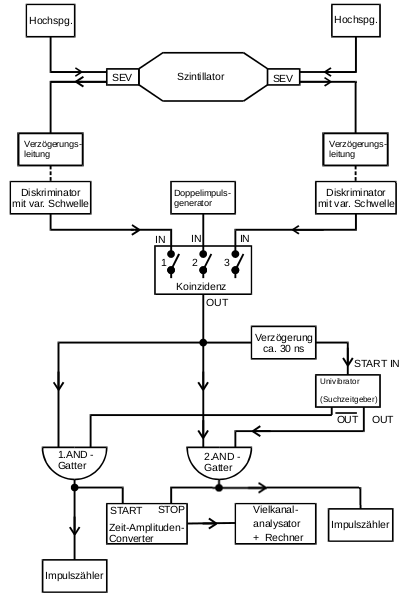
\includegraphics{Bilder/aufbau.png}
%	\label{fig:aufbau}
%\end{figure}
%
%\begin{figure}
%	\centering
%	\caption{Schematische Darstellung der Quelle zur Erzeugung radioaktiven Isotopen \cite{anleitung}.}
%	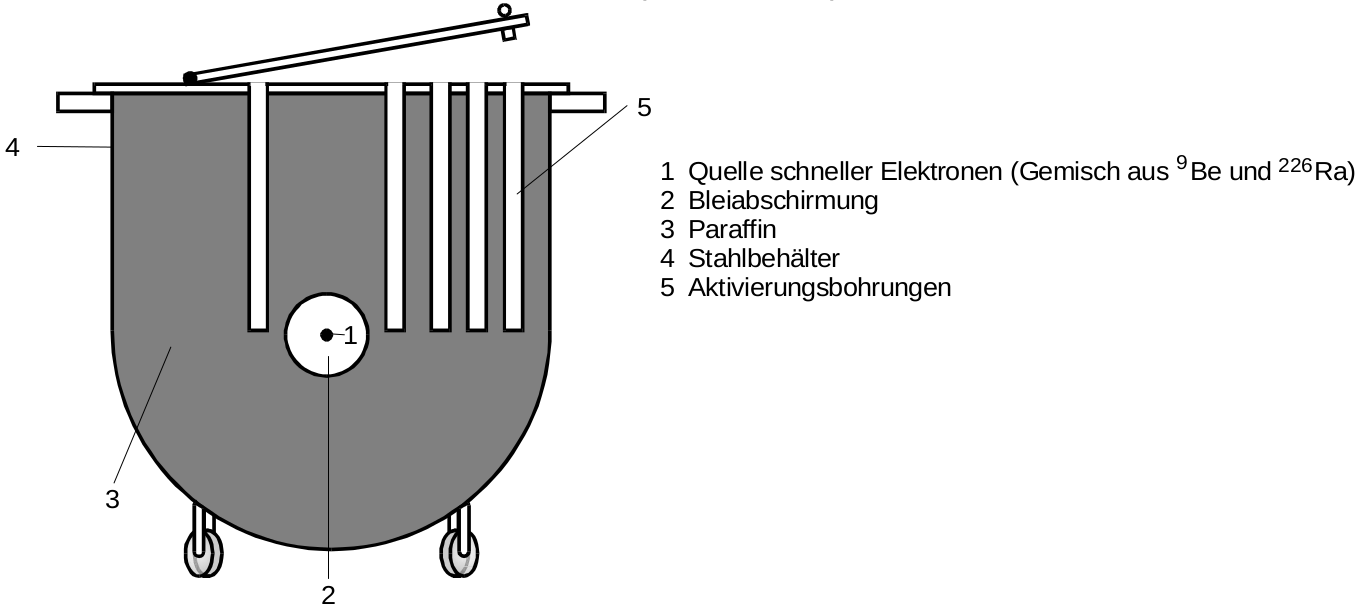
\includegraphics{content/toepfchen.png}
%	\label{fig:kochen}
%\end{figure}
%
Der Versuchsaufbau -- wie in Abbildung \ref{fig:aufbau} dargestellt -- besteht im Wesentlichen 
aus einem zerfallenden radioaktiven Isotop und einem Geiger-Müller-Zählrohr, welches die 
zerfallenden Kerne misst.
Das Geiger-Müller-Zählrohr ist entspricht einer mit Gas gefüllten Röhre. Trifft ein $\beta$-
oder $\gamma$- Teilchen auf ein Gasteilchen wird dieses ionisiert und kann aufgrund einer
anliegenden Spannung an der Röhre gemessen werden.
Dabei werden die gemessenen Zerfälle pro Messzeitintervall, welches am Zeitgeber einstellbar 
ist, an den Zählern 1 und 2 angezeigt. Nach jedem Messvorgang wird der Zähler umgeschaltet und 
der vorherige Wert auf dem aktuellen Zähler wird überschrieben. Der Versuchsaufbau ist mit
einer Blei-Abschirmung ausgestattet um die radioaktive Strahlung abzuschirmen.

Zur Erzeugung der radioaktiven Isotope wird das Objekt in Abbildung \ref{fig:kochen} verwendet.
Hierbei werden stabile Kerne mit niederenergetischen Neutronen beschossen. 
Da die Neutronen ihre Energie durch elastische Stöße an die Kerne übergeben und die maximale
Energie bei gleichen Massen der Stoßpartner erreicht wird, werden die Neutronen in einem 
Paraffinmantel gebremst, bis sie die optimale Energie besitzen.


\subsection{Versuchsbeschreibung}
\label{sec:Versuchsbeschreibung}
Zunächst wird der Acrylblock sowie die Fehlstellen mittels einer Schiebelehre vermessen.

Zur Bestimmung der Lage der Fehlstellen mit dem Impuls-Echo-Verfahren wird das Ultraschallechoskop über den Kippschalter auf den entsprechenden Messmodus (REFLEC.) gestellt.
Zunächst wird die tatsächlich auftretende Lauftzeit des Ultraschallsignals durch den Acrylblock bestimmt und mit dem theoretisch berechneten Wert verglichen, um die Dicke der Ausgleichsschicht bestimmen zu können.
Die Ultraschallsonde mit \SI{1}{\mega\Hz} wird mittels bidestillierten Wasser an den Acrylblock gekoppelt, welcher auf eine weiche Unterlage gestellt wird, um eine Beschädigung des Acrylblocks zu vermeiden.
An verschiedenen Stellen des Acrylblocks wird über einen \textbf{A-Scan} die Schalllaufzeit zur Ermittlung der Lage der Störstellen gemessen. Selbige Prozedur wird wiederholt, nachdem der Block umgedreht wurde und die Ultraschallsonde von der anderen Seite an den Acrylblock gekoppelt wurde.
\\Zur Untersuchung des Auflösungsvermögens wird eine Impuls-Echo-Messung mit der $\SI{4}{\mega\Hz}$-Sonde für die zwei nah nebeneinander liegende Störstellen (Fehlstellen 1\&2 in Abbildung \ref{fig:fehlstellen}) durchgeführt und mit den Ergebnissen der Messung mit der $\SI{1}{\mega\Hz}$-Sonde verglichen.
Die Ultraschallsonde wird hierfür erneut mittels bidestillierten Wasser an den Acrylblock gekoppelt.

Die Bestimmung der Lage der Fehlstellen wird zudem über den \textbf{B-Scan} realisiert. Hierzu wird die $\SI{1}{\mega\Hz}$-Sonde mittels bidestillierten Wassers an den Probenblock gekoppelt, die Aufnahme des \textbf{B-Scan} gestartet, und der Acrylblock wird mit der Ultraschallsonde langsam abgefahren.
Ebenso wie beim A-Scan wird die Messung bei umgedrehten Block wiederholt.

Zur Untersuchung des Herzmodells wird das obere Becherglas des herzmodells zu etwa einem Drittel mit bidestillierten Wasser gefüllt und die $\SI{1}{\mega\Hz}$-Sonde so auf der Wasseroberfläche positioniert, dass sie soeben eintaucht. Mittels eines Handblasebalg ist es möglich, Luft in das untere Becherglas zu pumpen, sodass sich die zwischen beiden Bechergläsern befestigte Gummimembran bewegt, der Abstand zwischen der Ultraschallsonde und der Membran somit verringert wird. Hierbei muss die Verstärkung so gewählt werden, dass die Signale  für beide Positionen der Gummimembran im \textbf{TM-Scan} deutlich zu sehen sind, zugleich aber auch nicht den Messbereich überschreiten.
Es wird ein \textbf{TM-Scan} mit $\SI{10}{\second}$ Laufzeit durchgeführt. Während der Messung wird der Handblasebalg möglichst gleichmäßig betätigt, um den Herzschlag zu simulieren.
